\documentclass{astroedu-lab}

\begin{document}

\pagestyle{plain}

\begin{problem}{\huge Лабораторная работа 5.1.2\\\\Эффект Комптона\\\\Выполнил Жданов Елисей Б01-205}

\section{Цель работы:}

С помощью сцинтиляционного спектрометра исследуется энергетический спектр $\gamma$-квантов, рассеянных на графите. Опреляется энергия рассеянных $\gamma$-квантов в зависимости от угла рассеяния, а также энергия покоя частиц, на которых происходит комптоновское рассеяние.

\section{Оборудование:}

Источник $\gamma$-квантов

Фотоэлектронный умножитель

АЦП, компьютер с ПО для визуализации

\section{Теоретическая справка}

Эффект Комптона -- увеличение длины волны рассеянного излучения по сравнению с падающим -- интерпретируется как результат упругого содуранеия двух частиц: $\gamma$-кванта и свободного электрона.
	
	Из закона сохранения 4-имульса для системы <<фотон + электрон>> следует формула для изменения длины волны рассеянного излучения:
	\begin{equation}
		\label{Kompton}
		\tag{$\star$}
		\Delta \lambda = \Lambda_K(1-\cos\theta),
	\end{equation}
	где величина $\Lambda_K = h/(mc) = 2,42 \cdot 10^{-10}$ см называется комптоновской длиной волны электрона.
	
	Из формулы (\ref{Kompton}) следует, что комптоновское смещение не зависит ни от длины волны первичного излучения, ни от рода вещества, в котором наблюдается рассеяние. В общем случае комптоновоское рассеяние происходит на свободных электронах в атоме. Для $\gamma$-квантов с энергией в несколько десятков, а тем более сотен килоэлектрон-вольт, связь электронов в атоме мало существенна, так как энергрия их связи в легких атомах не превосходит нескольких килоэлектрон-вольт, а для большинства электронов еще меньше.
	
	При рассеянии на связанных электронах изменение импульса кванта воспринимается атомом в целом. Посколько масса атома очень велика, переда ча импульса не спровождается сколь-нибудь заметной передачей энергии, и наблюдается несмещенная (по энергии) компонента в спектре рассеянного излучения. Таким образом, рассеяние $\gamma$-квантов на связанных электронах можно рассматривать как упругое столкновение квантов с атомами.
	
	Основной целью данной работы является проверка соотношения (\ref{Kompton}). Применительно к условиям нашего опыта формулу (\ref{Kompton}) следует преобразовать от длин волн к энергиям $\gamma$-квантов. Как нетрудно показать, соответсвующиее выражение имеет вид:
	\begin{equation}
		\label{1-cos}
		\tag{$\star\star$}
		\frac{1}{\varepsilon(\theta)} - \frac{1}{\varepsilon_0} = 1 - \cos \theta.
	\end{equation}

	Здесь $\varepsilon_0 = E_0/(mc^2)$ -- выраженная в единицах $(mc^2)$ энергия $\gamma$-квантов, падающих на рассеиватель, $\varepsilon(\theta)$ -- выраженная в тех же единицах энергия квантов, испытавших комптоновское рассеяние на угол $\theta$, $m$ -- масса электрона.
	
	Заменим в формуле~(\ref{1-cos}) энергию квантов, испытавших комптоновское рассеяние на угол $\theta$, номером канала $N(\theta)$, соответствующего вершине фотопика при указанном угле $\theta$:
	\begin{equation}
		\label{kek}
		\tag{$\star \star \star$}
		\frac{1}{N(\theta)} - \frac{1}{N(0)} = A (1- \cos \theta),
	\end{equation}
	где $A$ -- неизвестный коэффциицент пропорциональности между $\varepsilon(\theta)$ и $N(\theta)$.

\section{Экспериментальная установка}

%\begin{figure}[!h]
%	\centering
%	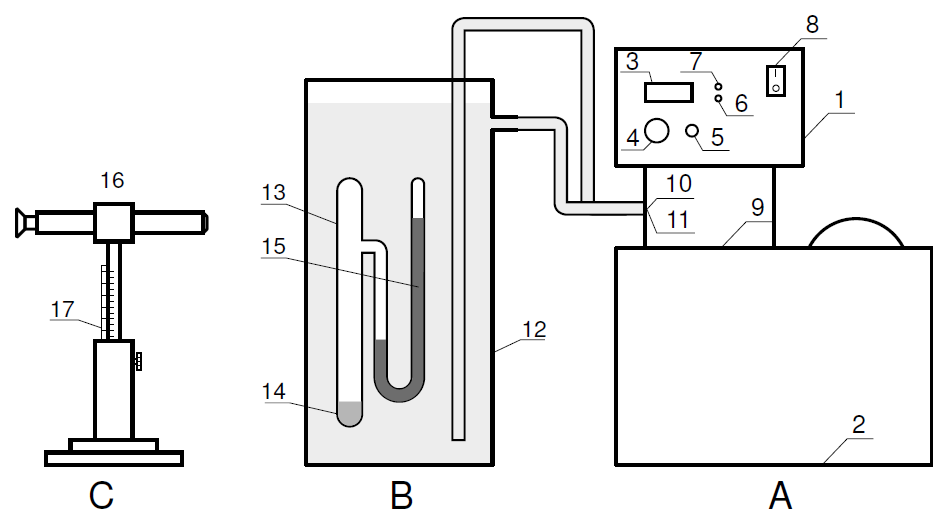
\includegraphics[width=0.9\textwidth]{установка.png}
%	\label{fig:boiler}
%\end{figure}

Техническая схема установки изображена на рис.1. Источником излучения 1 служит $^{137}$Cs, испускающий $\gamma$-лучи с энергией 662 кэВ. Он помещен в толстенный свинцовый контейнер с коллиматором. Сформмированный коллиматором узкий пучок $\gamma$-квантов попадает на графитовую мишень 2 (цилиндр диамтером 40 мм и высотой 100 мм.)




\begin{figure}[h] % Создаем плавающий объект для изображений
    \centering % Центрируем все содержимое
    \begin{minipage}[b]{0.45\textwidth}
        \centering
        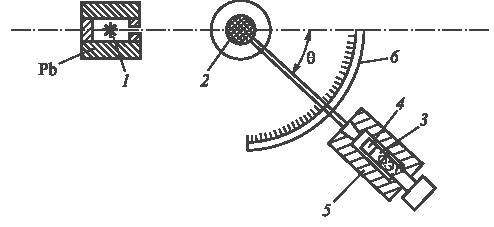
\includegraphics[width=\textwidth]{ustanovka1.pdf} % Вставляем первое изображение
        \caption{} % Подпись под изображением
    \end{minipage}
    \hfill
    \begin{minipage}[b]{0.45\textwidth}
        \centering
        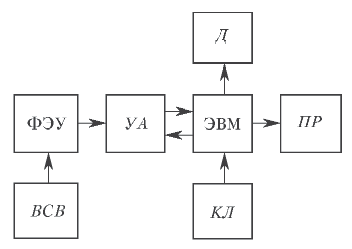
\includegraphics[width=\textwidth]{ustanovka2.pdf} % Вставляем третье изображение
        \caption{}
    \end{minipage}
    \caption{Установка}
\end{figure}

	
	Кванты, испытавшие комптоновское рассеяние в мишени, региструруются сцинтилляционным счетчиком. Счетчик состоит из фотоэлектронного умножителя 3 (далее ФЭУ) и сцинтиллятора 4. Сцинтиллятором служит кристалл NaI(Tl) цилиндрической формы диаметром 40 мм и высотой 40 мм, его выходное окно находится в оптическом контакте с фотокатодом ФЭУ. Сигналы, возникающие на ФЭУ, подаются на ЭВМ для амплитудного анализа. Кристалл и ФЭУ расположены в светонепроницаемом блоке, укрепленном на горизонтальной штанге. Штанга вместе с этим блоком может вращаться относительно мишени, угол поворота отсчитывается по лимбу 6.
	
	На рис.2 представлена функциональная блок-схема измерительного комплекса, который состоит из ФЭУ, питаемого от высоковольтного выпрямителя ВСВ, обеспечивающего работу ФЭУ в спектрометрическом режиме, усилителя-анализатора УА, являющегося входным интерфейсом ЭВМ, управляемой с клавиатуры КЛ. В ходе проведения эксперимента информация отражается на экране дисплея Д, окончательные результаты в виде таблиц и графиков могут быть выведены на принтер ПР.
	

\section{Измерения}

Продолжительность измерений разная - занесем её в таблицу, чтобы затем отнормировать $N$ на 100 секунд.

Довольно хороший способ регистрации истинной энергии пика - смотреть на пересечение его боковых сторон. Поскольку стороны пика близки к линиям в некоторой окрестности, с хорошей точностью, считая шумовой профиль также линейным, можно оценить реальную энергию.

Для регистрации числа отсчета выполняется вычитание измеренного шумового профиля с закрытым источнико(хотя с точностью до погрешности самого максимума $N$ это делать не так уж оправданно). 

Измерения приведены в электронной таблице, приложенной к работе.

%\begin{center}
%\begin{tabular}{|c|c|c|c|}
%\hline 
%\multicolumn{2}{|c|}{$h_\text{ман}$, мм} & $\sigma, \frac{\text{мН}}{\text{К}}$ & T, $^\circ$C \\
%\hline
%188.0 & 188.0 & $(64.5 \pm 3.9)$ & 22\\
%187.0 & 187.0 & $(64.0 \pm 3.9)$ & 30\\
%185.5 & 186.0 & $(63.3 \pm 3.9)$ & 35\\
%184.0 & 184.5 & $(62.5 \pm 3.9)$ & 40\\
%182.5 & 183.0 & $(61.7 \pm 3.9)$ & 45\\
%181.0 & 181.0 & $(60.8 \pm 3.8)$ & 50\\
%179.0 & 179.5 & $(59.9 \pm 3.8)$ & 55\\
%177.5 & 177.5 & $(59.0 \pm 3.8)$ & 60\\
%\hline
%\end{tabular}
%\end{center}

\section{Обработка}

Погрешность номера канала определяется не столько шириной пика, его дисперсией и временем выдержки, сколько неточностью выставления пунктирного указателя во время эксперимента и дальнейшей оцифровкой значений с использованием описанного выше метода. Для простоты разумно принять погрешность номера канала за 20 пунктов, тогда относительная погрешность составит $4\%$. Нанесем её размером точек на график.
\\
\begin{figure}[!h]
	\centering
	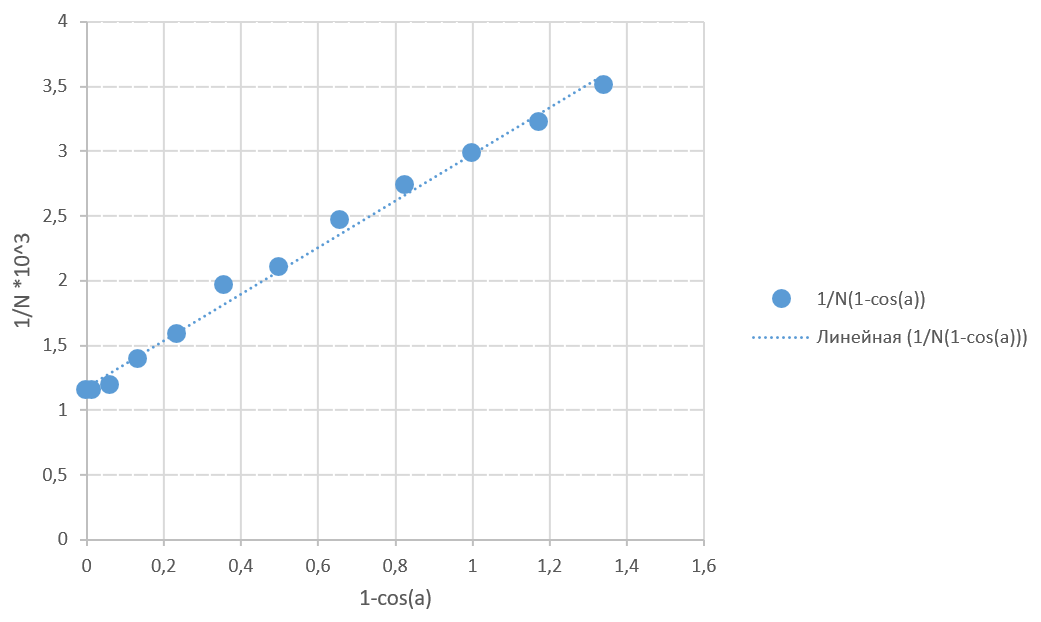
\includegraphics[width=1\textwidth]{граф.png}
	\label{fig:boiler}
\end{figure}

Найдем уравнение прямой(как видно, график линеаризован) для зависимости по МНК.

\[
	a = \frac{<x_i y_i> - < x > < y_i >}{< x_i^2> - < x_i >^2}
\]

\[
	b = < \nu_i > - a < N_i >
\]

Также рассчитаем её погрешности

\begin{equation}
	S_a^2 = \frac{< x_i^2>}{< x_i^2 > - < x_i >^2} \cdot \frac{<  b_i - b > ^2}{n - 2}
\end{equation}

Итоговое уравнение

\begin{equation}
	\frac{1}{N} = (a \pm S_a) + (b \pm S_b) \cdot (1 - \cos (\alpha)) = (1.174 \pm 0.035) + (1.803 \pm 0.051) \cdot (1 - \cos (\alpha)
\end{equation}

Подставим в уравнение $\alpha = 0 ^\circ$ и $\alpha = 90 ^\circ$ и получим значения

\begin{center}
	$N ( 0 ^\circ) = 850 \pm 30$\\
	$N ( 90 ^\circ) = 336 \pm 10$
\end{center}

Исходя из этих данных, по формуле (3) определим энергию покоя частицы, на которой происходит комптоновское рассеяние (по всем признакам -- электрон):
	\[m c^2 = E_\gamma \dfrac{N(90^\circ)}{N(0)-N(90^\circ)} = 662\cdot 10^3\times \dfrac{336}{850-336} = 430 \pm 50 \; \text{кэВ} \]
	
	



%\begin{center}
%	\Large $q(T)$
%\end{center}

%\begin{figure}[!h]
%	\centering
%	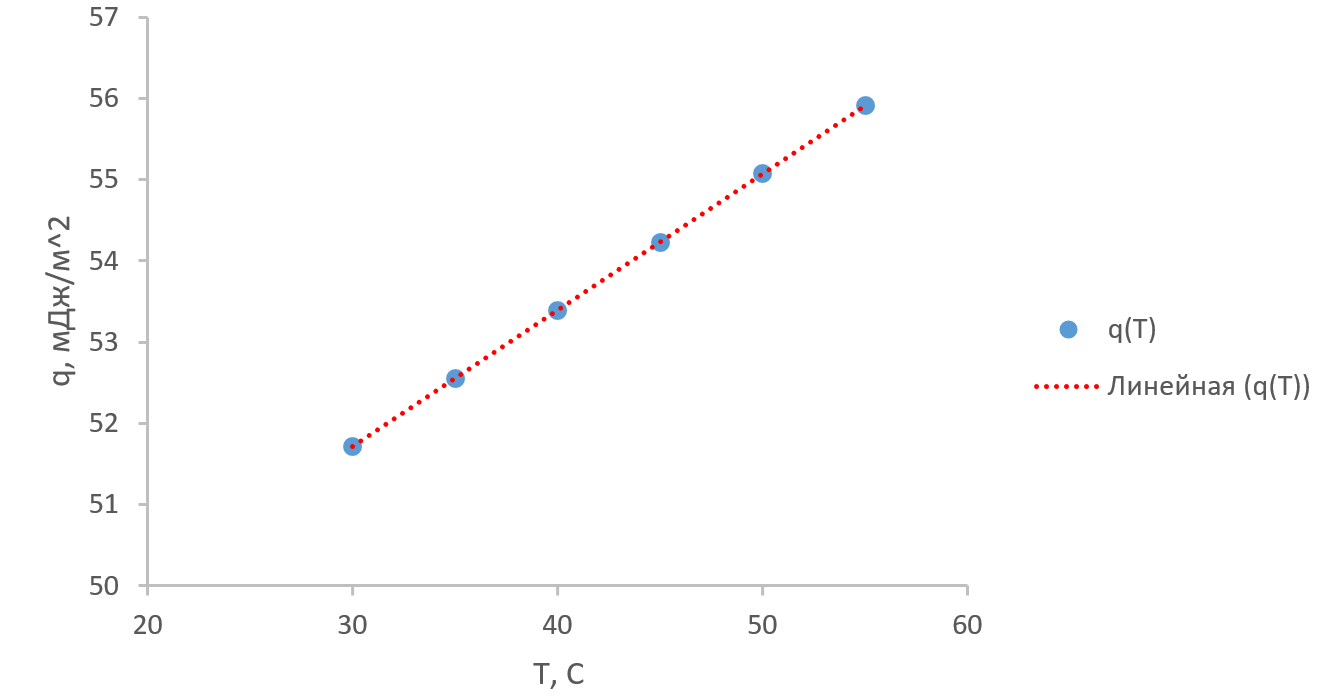
\includegraphics[width=1\textwidth]{2023-02-23_22-23-59.png}
%	\label{fig:boiler}
%\end{figure}

\section{Вывод}

Полученное значение $430 \pm 50 \; \text{кэВ}$ отличается от табличного значения энергии покоя электрона(511 кэВ), хоть и не сильно, что может быть связано как с неточным проведением эксперимента(требуется более точный метод отождествления максимума пика сигнала, и дальнейшая запись энергии), так и с тем, что электрон  в составе атома не является свободным, поэтому исходная формула не является достаточно точной в данном случае.

Тем не менее, был исследован энергетический спектр Комптоновского рассеяния $\gamma$-квантов на графите, определена масса покоя электрона. В электронной таблице дополнительно был построен график зависимости интенсивности излучения от угла рассеяния.

Итак, эффект Комптона был успешно зарегестрирован.




\section{Ресурсы}

Расчет по МНК: метод-наименьших-квадратов.рф


\end{problem}
\end{document}